\documentclass[]{report}

\usepackage{graphicx}
\usepackage{apacite}
\usepackage{natbib}
\usepackage[bottom]{footmisc}


% Title Page
\title{Keeping Functions Inline:\\An Eclipse Plug-in\\ Individual Requirements Analysis Document\\ \vspace{1cm} \texttt{https://github.com/mfraser4/comp195-spr19} \\ 
\includegraphics[width=3in]{imgs/eclipse_logo.png}}

% Authors
\author{Mark Fraser\\\texttt{m\_fraser3@u.pacific.edu}}


\begin{document}
\maketitle

\newpage
\tableofcontents
\newpage

\chapter{System Overview}

	\section{Basic Architecture}
	
		\begin{figure}[h!]
			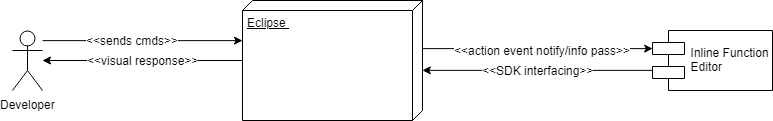
\includegraphics[width=\linewidth]{imgs/basic_architecture.png}
		\end{figure}
	
		This section is still in flux.  Initial analysis suggests that the plug-in will be an Eclipse workbench tool that interfaces with whatever current workspace environment the developer is in and the Eclipse UI.  Both of these can be represented as objects in code, and the project itself will be done in Java, an inherently Object-Oriented Programming language.  Thus, UML is an appropriate method to describe our project architecture once the software solution is better understood.  Eclipse plug-in development/SDK usage documentation is likely to be the single most important document required to derive an elegant solution for an inline/pseudo-inline function editor \citep{eclipseFoundation}.  Above is a basic architectural layout of our proposed plug-in.  Note that the plug-in is completely removed from the actor and only interfaces with Eclipse.  The user can access the plug-in's functionality, but only through the intermediary that is the foundational framework of Eclipse.
		
		Referencing the inter-woven nature of the use cases, the plug-in should support state machine functionality if some of the implied functionality of the use cases do not follow normal conventions.  This is proposed given the number of different paths with which use cases can be started.  Some use cases are not executed in isolation, and various efficiency-improvement functionality and error-handling should be implemented to handle these likely edge cases if possible within the time frame of this project.
	
	\section{Motivation}
	
		Software engineers' and programmers' services alike are in constant demand in today's technologically centered society.  Because there is insufficient supply to meet demand, software development personnel command higher salaries.  Thus, from a company's perspective, software engineers and programmers should be supported as much as possible to maximize their efficiency.  From the software engineer's and programmer's perspective, developing software should be as seamless a process as possible to facilitate implementing their code logic.  Many programmers develop in Integrated Development Environments (IDEs) to leverage shortcuts and plug-ins to streamline their workflow.  Eclipse is one of the most popular open-source IDEs with many plug-ins, but several key features are missing that have been implemented in other IDEs and are desired by developers.  Our goal is to implement one of these features:  inline function editing.
	
	\section{Purpose}
	
		The proposed plug-in will allow programmers to retain the context of the function they are currently developing while simultaneously viewing a called function's contents.  This will be done by displaying the called function's contents inline or pseudo inline with the calling function's contents.  Resultingly, fewer button presses, fewer mouse clicks, and less reorientation will be required for developers to work on two coupled functions.

\chapter{Current State of the Art}

	\section{Eclipse}
	
		Currently, Eclipse does not support inline function editing.  In order to view and edit a called function's contents (assumed to be in another file for this use case), the following steps are executed using keyboard shortcuts:
	
			\begin{enumerate}
				\item 
				Position cursor over called function
				
				\item
				Press $<$F3$>$
				
				\item 
				Current development pane shifts to called function's file
				
				\item
				Cursor is placed at function declaration
				
				\item 
				Developer makes changes to called function
				
				\item 
				$<$Ctrl+S$>$ to save contents
				
				\item 
				$<$Ctrl+W$>$ to close called function's editor pane
				
				\item 
				User is returned to original function pane
			\end{enumerate}
	
		Using mouse clicks, the following steps are required to perform the same action:
	
			\begin{enumerate}
				\item
				Position cursor over called function
				
				\item 
				Open \textit{Navigate} menu
				
				\item
				Select \textit{Open Declaration}
				
				\item
				Cursor is placed at function declaration
				
				\item 
				Developer makes changes to called function
				
				\item 
				Open \textit{File} menu
				
				\item
				Select \textit{Save} option
				
				\item 
				Click the "x" on the called function's editor pane
				
				\item 
				User is returned to original function pane
			\end{enumerate}

		This requires 8 and 9 steps, respectively.  Also, both use cases require the user to reorient themselves to a new editor pane.  If the developer needs to go back and forth between the files, this adds 3 steps for each iteration between:
		
			\begin{enumerate}
				\item
				Switching to other function editor pane
				
				\item
				Making changes/reviewing code
				
				\item 
				Switching back to original function editor pane
			\end{enumerate}

		This requires much overhead to view and/or edit two functions simultaneously.  Some might argue that one can simply place the editor panes side-by-side, but this use case requires one to clutter the screen with dense text, which is not desirable for a UI.  This will still diminish efficiency, as more text to process requires more of the user's energy to parse through.  As will be made clear in the following sections of other IDE's current implementations, inline function editing is the best use case of the three explored in this section.

	\newpage
	
	\section{Visual Studio 2017}

		Below is a snapshot from an instance of the inline function editor's usage:
		
		\begin{figure}[h!]
			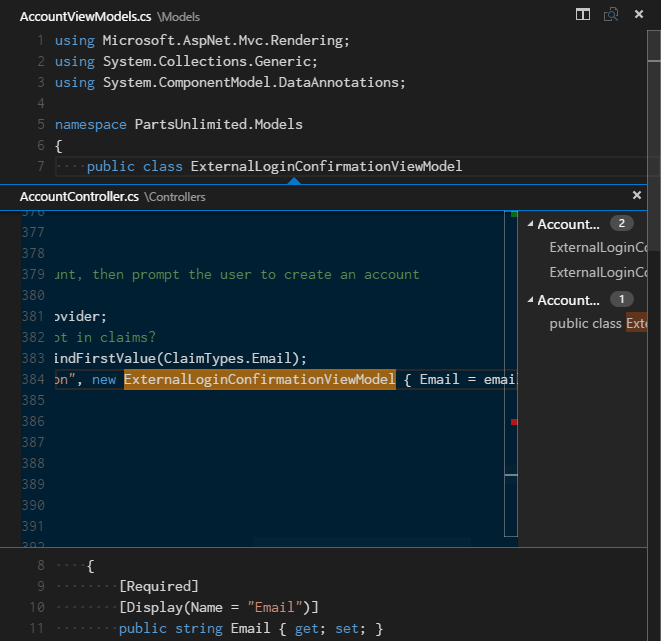
\includegraphics[width=\linewidth]{imgs/vs_peek_function.png}
		\end{figure}
		
		Visual Studio 2017 does support inline function editing through the following steps \citep{vsDownload}:

			\begin{enumerate}
				\item
				Position cursor over called function
				
				\item 
				Press $<$Alt+F12$>$
				
				\item
				Called function's file is opened to function's declaration within text below
				
				\item
				Cursor is placed at function declaration
				
				\item 
				Developer makes changes to called function
				
				\item
				$<$Ctrl+S$>$ to save contents
		
				\item 
				User clicks the "x" to close the called function editor box
			
				\item 
				The inline function editor box is closed, returning the pane to its original state
			\end{enumerate}
		
		One can observe benefits not necessarily clear, as the number of steps remains the same.  The function is opened within the pane.  Therefore, the only change from the user's perspective is a box of text opening beneath the called function, rather than an entirely new pane opening.  Also note that the original function can still be reviewed without any physical transitions.  Mental and physical overhead are not required to completely switch contexts between files.  Instead, the steps to switch between function editing is:
		
			\begin{enumerate}
				\item 
				Click outside inline function editor
				
				\item
				Making changes
				
				\item 
				Click inside inline function editor
			\end{enumerate}
		
		Clearly, this is a more seamless transition between the two functions than Eclipse currently possesses.
		
		There is one mark against Visual Studio.  Whether it be because it is poorly documented or simply unavailable, it appears a transition from the keyboard to the mouse and back is required to close the inline editor pane.  As a Vim and general non-IDE user looking to find a similar, yet more facilitated experience, this is a notable point of inefficiency and distraction.  In the proposed plug-in's implementation, the insertion of a keyboard hotkey to close the inline pane should be implemented if possible.

\chapter{Project Stakeholders}

	\section{Product Owner}
	
		The owner of the plug-in.  This stakeholder is responsible for delivering a product that meets the standards of Eclipse plug-ins and can be added to the plug-in store.  This stakeholder is also responsible for maintaining the integrity of the code base and managing possible pull requests from outside collaborators, as this project is open-source.
	
	\section{Client}
	
		Eclipse can be considered the client if it adopts this plug-in as a part of its plug-in store.  Eclipse is an open-source IDE, so it does not have any business stake except that it might receive more downloads if it possesses inline function editing.
	
		The University of the Pacific can also be considered a stakeholder in this project, as the success of this project can potentially be profitable in building the school's reputation in computer science by increasing U.o.P.'s presence in the computer science field.  The resulting product will also be displayed on Senior Project Day, so the SOECS will benefit from this product's success when displayed to the rest of the school.
	
	\section{Users}
	
		There is one general user of this plug-in, and that is users of Eclipse.  Eclipse users might be drawn to this IDE because of its low overhead costs compared to others (e.g. Eclipse requires only 360 MB storage and 3 MB of RAM to run, whereas Visual Studio requires 2.3 GB of storage and 250 MB of RAM).  The proposed plug-in contained herein provides similar functionality to comparable IDEs with substantially less overhead.
		
		There are no levels of privileges, as Eclipse is an open-source IDE, and there are no different levels of functionality to imply different clients (i.e. $-$ paid versus unpaid). Users of this plug-in will use it with the intention of increasing their development efficiency through better code navigation than what Eclipse currently offers.  Without any data to support this other than anecdotal evidence, keyboard-centric users might be more predisposed to utilize this functionality (e.g. Those experienced and most comfortable with Vi, Emacs, and other similar terminal editors).

\chapter{Non-Functional Requirements}

	\section{Constant Uptime}
	
		Users should be able to access this functionality at any time that Eclipse is open.  The plug-in must inherently be stable to achieve this requirement.
	
	\section{Efficiency and Minimalism}
	
		The plug-in's usage should match its purpose, which is to improve efficiency of code viewing and editing.  Thus, the interfacing mechanisms involved should be implemented with minimal effort on the developer's side, both mentally (memorizing hotkeys, switching editor panes, et ceters) and physically (key strokes, keyboard-to-mouse movements, and vice/versa).
		
		Developers are most efficient when utilizing a consistent method of human-computer interaction.  Of the available tools, the keyboard is the most efficient interface, as most all developer tools have been created with keyboard hotkeys, and manually generated code is created via the keyboard.  Also, developers are very likely to spend time interfacing through CLI with other devices, so consistency is key.  This is opposed to switching between using the keyboard and mouse, or keyboard and touchscreen, or all of the above.  Thus, a plug-in dedicated to efficiency should therefore provide some hot key functionality on the keyboard to best fulfill its goal.
	
	\section{Multiple Paths of Execution}
	
		For developers who do not wish to bind this plug-in's functionality to the main use case(s), they must still be able to interface with the plug-in through the Eclipse menus.  Therefore, menu options and/or other usage cases must be implemented to guarantee interfacing functionality.
	
	\section{Efficient Content Display}
	
		The plug-in's purpose is to display text inline or pseudo inline with the current file to increase developer efficiency.  Thus, the contents of the function to be displayed must be shown in an efficient manner such that users can easily switch between the called function's contents and the calling function's contents.
	
	\section{Failure Management}
	
		Some functions might not exist or be findable.  Proper error-handling and user informing should be established to effectively communicate this to the user.
	
	\section{Portability}
	
		Referring to portability between Eclipse versions.  The plug-in should be architected to maintain functionality and require minimal changes when ported to future versions of Eclipse.
	
\chapter{Functional Requirements}
	
	\section{Use Case Diagram}
	
		The use cases described in the diagram on the following page can be argued to be part of one overall larger use case, which is editing called functions inline with the original function.  However, given the high focus on efficiency, a finer granularity is required to identify how to best execute this overall use case with the minimum amount of key strokes/button presses and the most intuitive interfacing methods.  Also, do misinterpret minimalist use case descriptions/steps to result from a desire to minimalize functionality.  Rather, these steps are born from a desire to simplify and minimalize the plug-in's presence.  It's goal is to facilitate development, not come under the spotlight of users.  This implies that more work will have to be performed on the plug-in's backend functionality to best facilitate these use cases.
	
		\begin{figure}[h!]
			\centering
			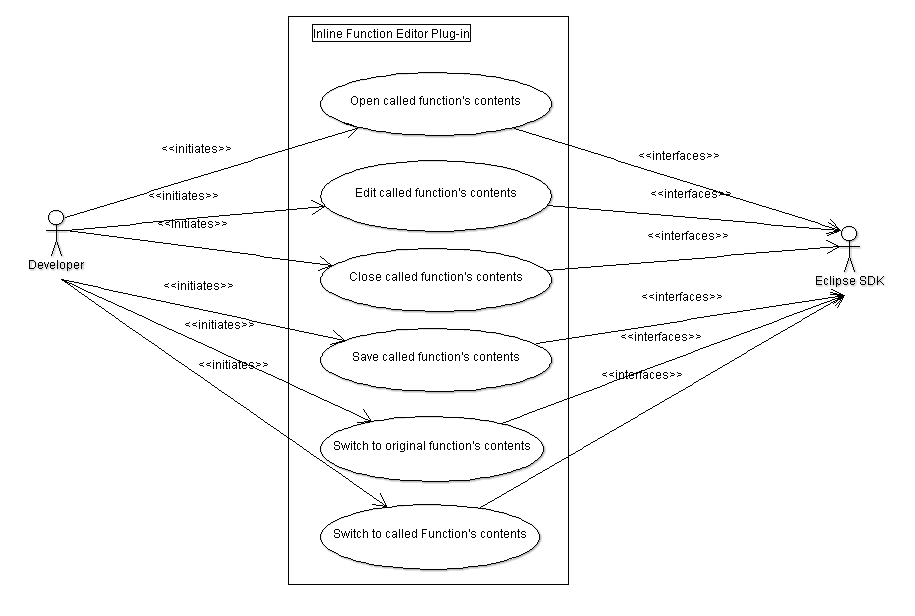
\includegraphics[width=\linewidth]{imgs/use_case_diagram.png}
		\end{figure}
	
	\newpage
	
	\section{Casual Use Case Descriptions}
	
		\subsubsection{UC1:  Open called function's contents}
		
			The user, upon positioning his cursor over the called function, can open either the \textit{Navigate} menu and select a "Peek Function" option, or press some keyboard hotkey (preferably one button).  An editor pane contained within the original pane should open with the called function's file opened to the declaration of the called function.  If the called function is declared within the same file, a duplicate of the file should be opened, but synchronicity should be maintained between the two versions of the file to avoid race conditions.  Perhaps for version 0.0, this functionality should be prevented, as this is the most complicated use case, or at least documented to be unsupported.  A warning label could be shown to notify the user of possible error in editing the same content between two panes. If the function is recursive and calls itself, it might be most prudent to disallow this functionality as well for version 0.0.  Also, if the user attempts to press the same hotkey on a called function within a called function's editor, the plug-in should go to \textbf{UC3}.  Supporting nested inline editors opens many complicated use cases and alternate states.  Upon the completion of this use case, \textbf{UC1}, \textbf{UC5} should follow naturally.
			
		\subsubsection{UC2:  Edit called function's contents}
		
			An implied use case for this plug-in.  This use case should be satisfied following standard Eclipse document editing to mesh with the general Eclipse workflow.  For example, clicking, keyboard navigation, typing, et cetera, should all be supported.  There is a possible race condition of this file being opened in a separate editor pane and the user making unsaved changes to this file first.  If possible, a file listener should know when changes are made and be reflected in the inline plane, if possible, or make the user refresh the file and reapply his changes.
		
		\subsubsection{UC3:  Close called function's contents}
		
			Once the user has completed whatever his purpose for opening the called function's declaration, he should be able to close the inline editor pane.  This should be supported at least two ways:  keyboard and an "x" button.  If the file has been modified but not saved, \textbf{UC4} should be consulted first.  This use case and, if applicable, \textbf{UC4} should be consulted if the original editor pane is closed.  \textbf{UC4} should be executed upon the completion of this use case.
			
		\subsubsection{UC4:  Switch to original function's contents}
		
			An implied use case for this plug-in.  Leveraging the Eclipse SDK UI components should automatically allow for this functionality.  This use case is dependent on the user being in the called function's editor pane.   This use case should also be executed upon the completion of \textbf{UC3}.
			
		\subsubsection{UC5:  Switch to called function's contents}
		
			An implied use case for this plug-in.  Leveraging the Eclipse SDK UI components should automatically allow for this functionality.  This use case is dependent on the user being in the original function's editor pane.  This use case should also be executed upon the completion of \textbf{UC1}.  If it is executed as a result of \textbf{UC1}, the cursor should preferably be placed at the function declaration line.
	
	\section{Fully Dressed Use Case Descriptions}
	
		\subsubsection{UC1: Open called function's contents}
		
			\textbf{Preconditions:}
			
				\begin{enumerate}
					
					\item Cursor positioned over word in open file
					
					\item No other inline pane is open
					
				\end{enumerate}
		
			\noindent\textbf{Use Case Scenario:}
			
				\begin{enumerate}
					
					\item
					User makes call to open inline function editor
					
						\subitem
						User presses associated keyboard hotkey
						
						\subitem
						User goes to \textit{Navigate} menu option and clicks on associated sub-option
					
					\item 
					If valid function located in separate file, go to step 3, else 6
					
					\item
					Eclipse editor pane opens
					
					\item 
					\textbf{UC5}
					
					\item 
					Go to end
					
					\item
					Display error message corresponding to following conditions:
					
						\subitem
						If not a valid function (e.g. undeclared, variable, et cetera), display to user that function could not be found
						
						\subitem 
						If function is declared within file, display to user that functions declared within document cannot be edited inline (perhaps suggest they press $<$F3$>$ instead to jump to declaration)
						
						\subitem
						If the called function is the same as the original function, display to user that recursive function calls cannot be edited inline
						
						\subitem
						Display to user an unknown error has occurred
					
					\item 
					End
					
				\end{enumerate}
			
			\noindent\textbf{Postconditions:}
			
				\begin{enumerate}
					
					\item 
					None
					
				\end{enumerate}
			
		\vspace{0.25in}
			
		\subsubsection{UC2:  Edit called function's contents}
		
			\textbf{Preconditions:}
		
				\begin{enumerate}
					
					\item \textbf{UC1}
					
					\item Cursor is located within inline editor pane
					
				\end{enumerate}
		
			\noindent\textbf{Use Case Scenario:}
			
				\begin{enumerate}
					\item
					User makes changes in accordance with standard Eclipse functionality to navigate and edit text
					
					\item
					End
				\end{enumerate}
			
			\noindent\textbf{Postconditions:}
			
				\begin{enumerate}
					
					\item 
					None
					
				\end{enumerate}
			
		\vspace{0.25in}
		
		\subsubsection{UC3:  Close called function's contents}
		
		\textbf{Preconditions:}
		
		\begin{enumerate}
			
			\item \textbf{UC1}
			
		\end{enumerate}
		
		\noindent\textbf{Use Case Scenario:}
		
		\begin{enumerate}
			\item
			User presses the hotkey to open the called function
			
			\item 
			If file contents have been changed, prompt user to ask if they wish to save new version of file.
			
			\item
			If user answers "yes," go to step 4, else go to step 5
				
			\item 
			Save inline editor contents to file on disk
			
			\item 
			If cursor is located within inline editor pane, \textbf{UC4}
			
			\item 
			The inline editor pane closes
			
			\item
			End
		\end{enumerate}
		
		\noindent\textbf{Postconditions:}
		
		\begin{enumerate}
			
			\item 
			None
			
		\end{enumerate}
		
		\vspace{0.25in}
		
		\subsubsection{UC4:  Switch to original function's contents}
		
		\textbf{Preconditions:}
		
		\begin{enumerate}
			
			\item \textbf{UC1}
			
		\end{enumerate}
		
		\noindent\textbf{Use Case Scenario:}
		
		\begin{enumerate}
			
			\item 
			If resulting from \textbf{UC3}, jump to step 3
			
			\item
			User uses one of the following methods to switch to original function's contents:
			
				\subitem
				Standard mouse click to switch to original editor pane
				
				\subitem
				An intuitive variant of hotkey that handles open/close functionality (e.g. $<$Ctrl+Hotkey$>$)
			
			\item 
			The cursor is repositioned within the original function editor pane
			
				\subitem
				If resulting from \textbf{UC3}, cursor defaults to called function's location in original function
			
				\subitem
				If done via mouse click, cursor should reposition to wherever mouse identifies, as is standard with text editors
				
				\subitem
				If done using a hotkey, cursor defaults to called function's location in original function
			
			\item
			End
		\end{enumerate}
		
		\noindent\textbf{Postconditions:}
		
		\begin{enumerate}
			
			\item 
			None
			
		\end{enumerate}
		
		\vspace{0.25in}
		
		\subsubsection{UC5:  Switch to called function's contents}
		
		\textbf{Preconditions:}
		
		\begin{enumerate}
			
			\item \textbf{UC1}
			
			\item \textbf{UC4} (unless resulting from \textbf{UC1})
			
		\end{enumerate}
		
		\noindent\textbf{Use Case Scenario:}
		
		\begin{enumerate}
			
			\item 
			If resulting from \textbf{UC1}, jump to step 3
			
			\item
			User uses one of the following methods to switch to called function's contents:
			
				\subitem
				Standard mouse click to switch to inline editor pane
				
				\subitem
				An intuitive variant of hotkey that handles \textbf{UC1}, \textbf{UC3} functionality (e.g. $<$Ctrl+Hotkey$>$)
			
			\item 
			The cursor is repositioned within the inline function editor pane
			
				\subitem
				If resulting from \textbf{UC1}, cursor defaults to called function's declaration within inline editor
				\subitem
				If done via mouse click, cursor should reposition to wherever mouse identifies, as is standard with text editors
				
				\subitem
				If done using a hotkey, cursor defaults to called function's declaration within inline editor
				
					\subsubitem
					If \textbf{UC5} has been previously executed and development time allows, cursor should be returned to last location within inline editor
			
			\item
			End
		\end{enumerate}
		
		\noindent\textbf{Postconditions:}
		
		\begin{enumerate}
			
			\item 
			None
			
		\end{enumerate}

\chapter{Sequence Diagrams}

	At this stage of development, sequence diagrams will be expressed at a conceptual level.  Several preliminary sequence diagrams are shown below to illustrate the most crucial use cases.
	
	\begin{figure}[h!]
		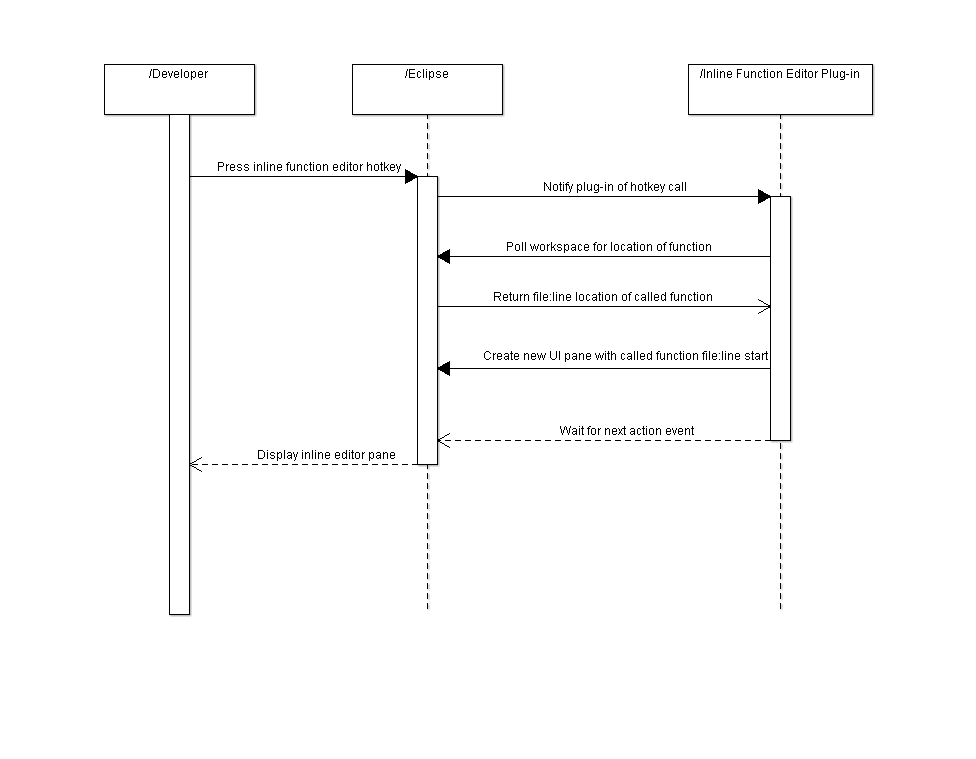
\includegraphics[width=\linewidth]{imgs/open_editor.png}
		\caption{Open inline function editor}
	\end{figure}
	
	\begin{figure}[h]
		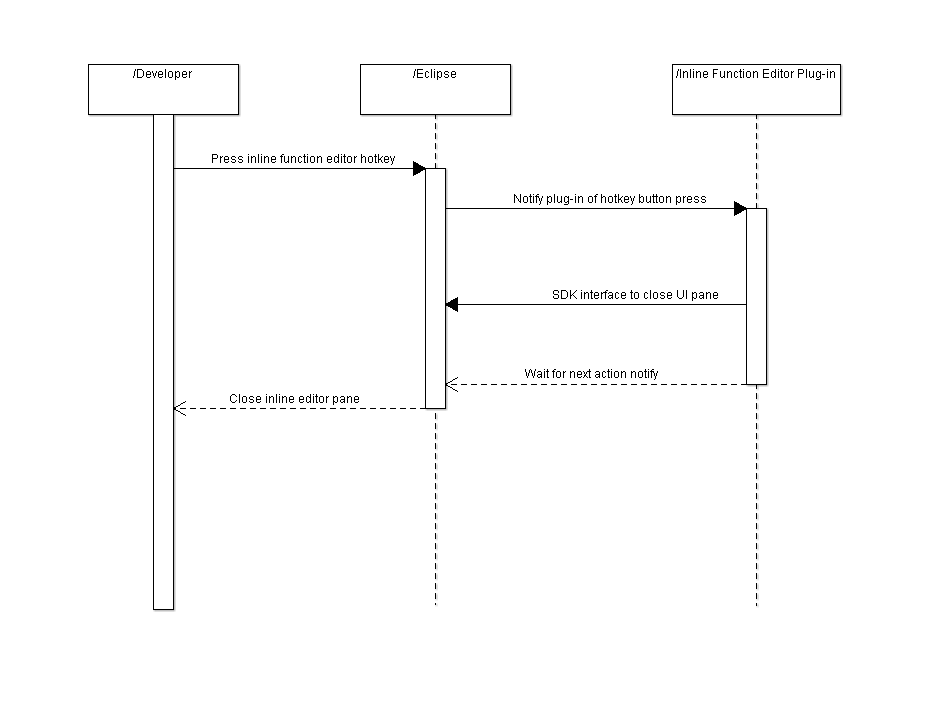
\includegraphics[width=\linewidth]{imgs/close_editor.png}
		\caption{Close inline editor pane}
	\end{figure}

	\begin{figure}
		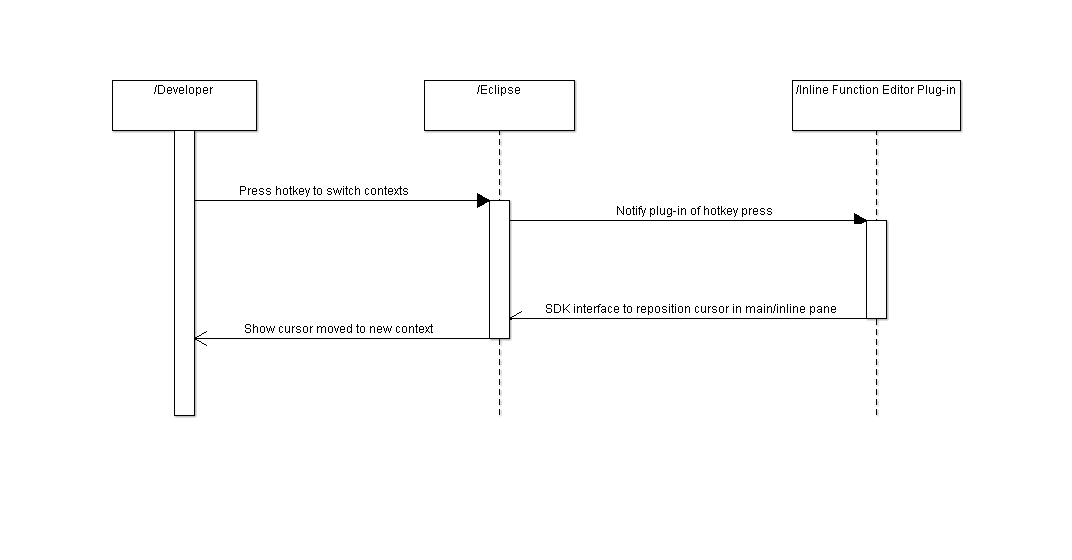
\includegraphics[width=\linewidth]{imgs/switch_context.png}
		\caption{Switch editor pane contexts}
	\end{figure}

\chapter{UI Design}

	Below is an initial mock-up of our design.  Given the architecture of Eclipse, creating a pseudo-inline editor pane tied to the location of the called function is the current path of least resistance, but this may be subject to change as the development continues.  Implementing a literal inline function editor like Visual Studio would require the functionality be built into the editor panes, which goes beyond the scope of a plug-in developed over a few months.  Creating an individual instance of a pane with the file opened to the declared function should still take the same number of steps as an inline function editor like Visual Studio's.

	\begin{figure}[h!]
		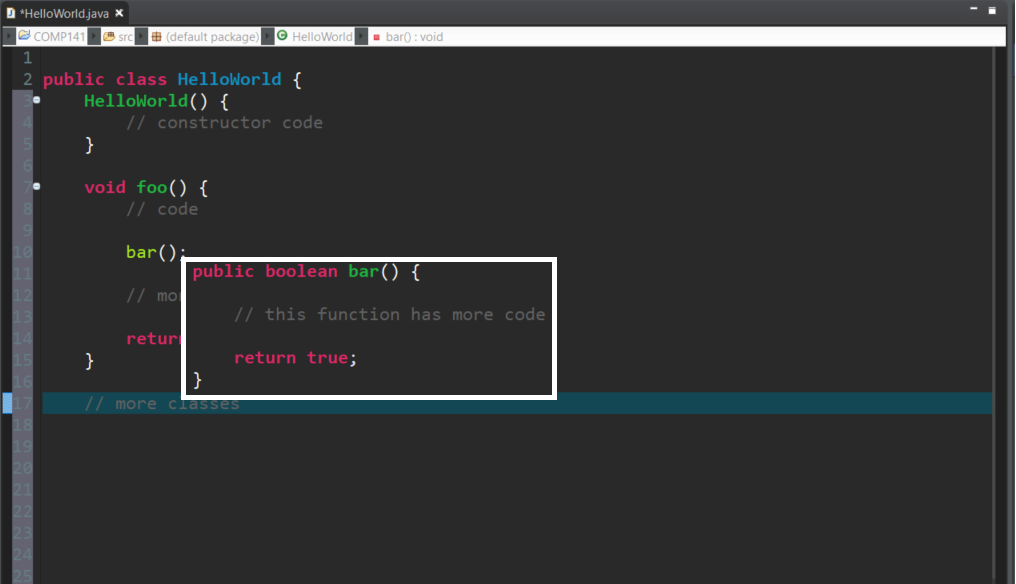
\includegraphics[width=\linewidth]{imgs/ui_mockup.png}
	\end{figure}



\chapter{Glossary of Terms}

	\noindent\textbf{Eclipse}\\ \\
	Eclipse is an integrated development environment (IDE) used in computer programming, and is the most widely used Java IDE.  It contains a base workspace and an extensible plug-in system for customizing the environment \citep{eclipse}. \\ \\

	\noindent\textbf{Hotkey}\\ \\
	A keyboard shortcut (e.g. $<$F3$>$).\\ \\
	
	\noindent\textbf{Inline Function Editor}\\ \\
	An instance of an editor that is opened "inline" with the original text.  See the chapter "UI Design" for graphical aids.  For the purposes of this RAD, an inline function editor is considered an editor pane contained within the originating editor pane.\\ \\

	\noindent\textbf{Integrated Development Environment (IDE)}\\ \\
	An integrated development environment (IDE) is a software application that provides comprehensive facilities to computer programmers for software development. An IDE normally consists of a source code editor, build automation tools, and a debugger. Most of the modern IDEs have intelligent code completion \citep{ideWiki}.\\ \\
	
	\noindent\textbf{Open-Source}\\ \\
	Open-source software (OSS) is a type of computer software in which source code is released under a license in which the copyright holder grants users the rights to study, change, and distribute the software to anyone and for any purpose \citep{oss}.
	
	\noindent\textbf{Pane}\\ \\
	A section of a window that provides the user with additional information or quick access to features commonly used in a software program \citep{pane}.
	
	\noindent\textbf{Plug-in}\\ \\
	In computing, a plug-in (or plugin, add-in, addin, add-on, or addon) is a software component that adds a specific feature to an existing computer program \citep{plugIn}. \\ \\

%%%%%%%%%%%%%%%%%%%%%%%%%%%%%%%%%%%%%%%%%%%%%%%%%%%%%%%%%%%%%%
%% 					BIBLIOGRAPHY							%%
%%%%%%%%%%%%%%%%%%%%%%%%%%%%%%%%%%%%%%%%%%%%%%%%%%%%%%%%%%%%%%
\bibliographystyle{apacite}
\raggedright
\bibliography{mybib.bib}

\end{document}
